% Ubah judul dan label berikut sesuai dengan yang diinginkan.
\section{Design and Implementation}
\label{sec:designandimplementation}

% Ubah paragraf-paragraf pada bagian ini sesuai dengan yang diinginkan.
This research is explaining about the implementation of one of the branch of deep learning studies with the aim to automatically detect Indonesian hoax news by leveraging BERT method. This detection method is trained by using a combination of dataset from \url{https://data.mendeley.com/datasets/p3hfgr5j3m/1} and dataset that we made ourself for this paper alone by using web crawling technology. Picture \ref{fig:metodologi} is the outline of this research in a nutshell.

\begin{figure} [h!]
    \centering
    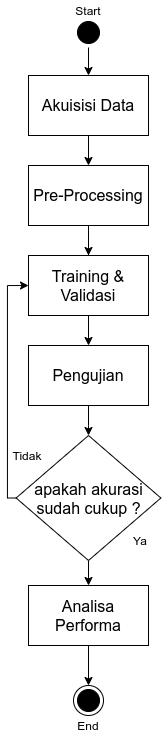
\includegraphics[width=0.3\columnwidth]{gambar/metodologi_vertical.png}
    \caption{This research method in a nutshell.}
    \label{fig:metodologi}
\end{figure}

\subsection{Material and Tools Specification}

The dataset that is being used in this research is a dataset originated from \url{https://data.mendeley.com/datasets/p3hfgr5j3m/1} coupled with our own made dataset in which we have create it using web crawling technology. Both of these dataset combined, is resulting in total of 1621 data with the exact details can be seen at table \ref{tab:dataset}. Meanwhile, table \ref{tab:dataset_mendeley} is the starting point of our dataset which we gotten from \url{https://data.mendeley.com/datasets/p3hfgr5j3m/1} alone.

Each of these dataset is containing the content of the news along with its label which can be either "Valid" or "Hoaks". We took the news from accredited and verified news sources for the valid news, while on the other side, we took all of the hoax news mostly from \url{https://turnbackhoax.id}, a website that contains the list of user reported hoax news from many sources.

\begin{table}[h]
    \caption{Total of news from \url{data.mendeley.com}}
    \label{tab:dataset_mendeley}
    \centering
    \begin{tabular}{ | l | l | }
        \hline
        \textbf{Label} & \textbf{Total Data} \\ \hline
        \textit{Hoaks} & 228                 \\ \hline
        \textit{Valid} & 372                 \\ \hline
        \textbf{Total} & \textbf{600}        \\ \hline
    \end{tabular}
\end{table}

\begin{table}[h]
    \caption{Total of training dataset}
    \label{tab:dataset}
    \centering
    \begin{tabular}{ | l | l | }
        \hline
        \textbf{Label} & \textbf{Total Data} \\ \hline
        \textit{Hoaks} & 885                 \\ \hline
        \textit{Valid} & 736                 \\ \hline
        \textbf{Total} & \textbf{1621}       \\ \hline
    \end{tabular}
\end{table}


\begin{table}[h]
    \caption{Dataset Sample}
    \label{tab:contoh_dataset}
    \centering
    \begin{tabular}{ | p{.8\linewidth} | l | }
        \hline
        \textbf{news}                                                                                                                                                                                                                     & \textbf{tagging} \\ \hline
        Wakil Gubernur DKI Jakarta Sandiaga Uno menargetkan pengerjaan tahap awal Stadion BMW dilakukan pada Oktober. Stadion ini diperuntukkan bagi klub Persija....                                                                     & Valid            \\ \hline
        "Komisi II bersama KPU dan Bawaslu masih membahas ketentuan wajib cuti bagi petahana presiden yang maju Pilpres 2019. Mekanisme pengambilan.....                                                                                  & Valid            \\ \hline
        Jaksa penuntut Ulumum (JPU) pada Komisi Pemberantasan Korupsi (KPK) mencecar Pejabat Pembuat Komitmen (PPK) reguler pada Direktorat Perlindungan Sosial Korban Bencana Sosial Kemensos Victorious Saut Hamonangan Siahaan soal... & Valid            \\ \hline
        “Halo Kak! Aku Winda Dari Team Giveaway BAIM WONG Anda Memenangkan Hadiah Uang 100Jt dari kami info klik: https://wa.me/+6285796306857”                                                                                           & Hoax             \\ \hline
        “Apa yang terjadi dengan hewan dalam penelitian?   Teknologi ini telah dicoba pada hewan, dan pada hewan penelitian yang dilakukan, semua hewan mati , tidak langsung dari suntikan...                                            & Hoax             \\ \hline
        “Kadrun istilah dr PKI alias KOMUNIS ditujukan buat islam. Kl mau jd komunis pake aja istilah kadrun buat umat islam. Auto lsg Komunis”                                                                                           & Hoax             \\ \hline
    \end{tabular}
\end{table}

\subsection{Data Acquisition}

Because the dataset that we get from \url{https://data.mendeley.com/datasets/p3hfgr5j3m/1} feel severely lacking for our purpose because it only consist of 600 data, and because there are no web crawling which outputting its result into a convenient CSV file from Indonesian news sites, we took on our hand a task to create a webcrawling program to take news content from many Indonesian news sites, those sites included but not limited to \url{liputan6.com}, \url{detik.com}, \url{tempo.com} and others. As all of those sites is rightfully accredited and verified by the government, it is used for our valid news dataset. Our hoax news site however, only has one source from \url{turnbackhoax.id}, this is mainly because said site has quite an active forum behind it in which lots of people can report their finding of hoax text, seen and checked by lots of other people, before lastly, will be uploaded to the \url{turnbackhoax.id} site. But, the biggest factor in choosing that site compare to others is mainly because \url{turnbackhoax.id} wrote the original hoaxes text in their website, this coupled with the fact that their website has some kind of structure into it has shorten our task significantly. For this research, the webcrawling process has took news from varied dates, ranging from April 2018 as the oldest to April 2021.

\begin{figure} [h!]
    \centering
    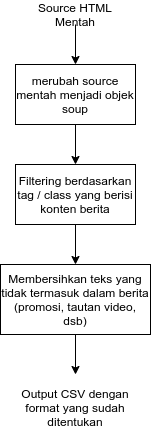
\includegraphics[width=0.35\linewidth]{gambar/webcrawl_long.png}
    \caption{Garis besar alur program \textit{web crawl}.}
    \label{fig:webcrawl_method}
\end{figure}

Picture \ref{fig:webcrawl_method} is the outline flow of the webcrawling program. Starting with inputting raw HTML code into the program, changing said code into an easier-to-process objects, get the news text and do some post-cleaning on the text, lastly, create a .CSV file to store all of the obtained news text with the appropriate format.

\begin{lstlisting}[
    language=HTML, 
    caption={Penggalan Kode Sumber HTML \url{detik.com}.},
    label={lst:source_detik}
]

...
<div class="detail__body itp_bodycontent_wrapper">
<div class="detail__body-text itp_bodycontent">

<strong>Jakarta</strong> - Koalisi <a href="https://
detik.com/tag/jokowi" target="_blank">Jokowi</a> 
sedang menyusun visi-misi jagoannya. Setelah 
menerima masukan dari <a href="https://detik.com/
tag/muhammadiyah" target="_blank"> Muhammadiyah</a>,
 ... 
Dan kita pun membuka diri untuk menerima 
masukan untuk penyempurnaan," imbuhnya.<br><br><!--
s:parallaxindetail--><div class="clearfix"></div><style>
...

\end{lstlisting}

Firstly, we need to determine tag or class of the HTML code for our first filter. If we look into listing \ref{lst:source_detik} as a reference, we can see \texttt{detail\_\_body\-text} class is the one that containing our desired news text. We filtered that class by inputting the class name into the appropriate parameter.

More often than not, our filtering result will contain some garbage or unrelated text resulting in the need to refine it further by post-clean it after the filter process. Usually, those text is writer or editorial notes, ad, or related news links which we don't need at all.

Finally, the last step is outputting all of the acquired news text as a .CSV file. There are no particular reason on the article of why we chose CSV file format compared to other famous file format aside from the CSV file format is easier to use in our training program and because it is an open-format that can be opened and edited if need be, by nearly any spreadsheet program.

As the general interface and improving user experience for our webcrawling software, we use a .json format file to configure what news sources that we want to get, how much is it, and when is it. All of those configuration will be processed by the program and the program will take the news in accordance with said configuration.

\subsection{Preprocessing}

\begin{figure}[h!]
    \begin{center}
        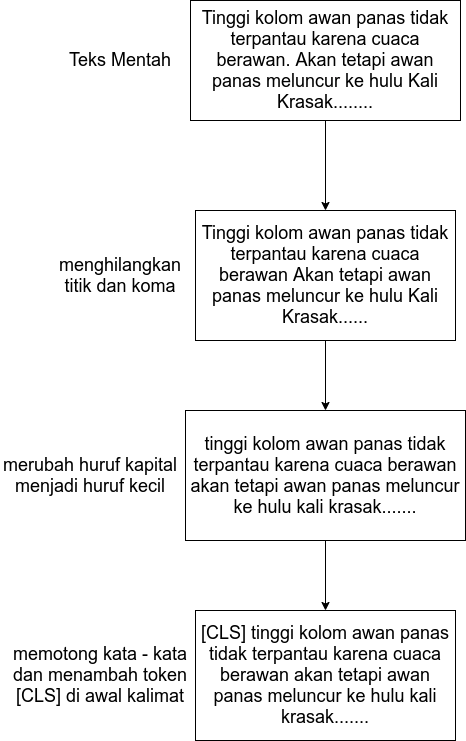
\includegraphics[width= .7\linewidth]{gambar/preprocess_long.png}
        \caption{Preprocessing Method}
        \label{fig: metodologi_preprocessing}
    \end{center}
\end{figure}

In this particular process, data need to be prepared first thing before being processed into BERT. This data preprocessing method is consisted of removing any punctuation in the text, change all of the capital letter into its lower letter and truncate any texs that is longer than the capacitites of word that BERT could process at once that is at 512 words or token. There are a few options on how to truncate the text, for example we can take the first 512 words and delete the rest, we can take the last 512 words, or we can combine from both the start of the text and the end portion of the text with some ratio. Last step of this preprocessing is to add a special \texttt{[CLS]} token. Picture \ref{fig: metodologi_preprocessing} will explain the same thing but with a better clarity.

Other than that, we will also divide the dataset into 3 portionss with details stated below :

\begin{itemize}
    \item 70\% Training, 10\% Validation, 20\% Test
\end{itemize}

\begin{enumerate}
    \item Training

          This set is used with BERT as an input when it is in its training phase so we can get an optimized model for our task.

    \item Validation

          This set is used right after BERT finished its training phase. Used to determined whether our created model has appropriate weight for our task or if our model still need to be trained again. This portion is also used to determine whether our model is overfitting or underfitting which is a bad thing.

    \item Test

          This set is used as an accuracy test after both the validation and the training phase is finished. The resulting accuracy of this set is the one that we consider as our result.

\end{enumerate}

To make it clearer, check table \ref{tab:dataset_section}. We can see based on this table that the divition of the dataset is already appropriate.

\begin{table}[h]
    \caption{Dataset Portioning Details}
    \label{tab:dataset_section}
    \centering
    \begin{tabular}{ | l | l | l | l | }
        \hline
        \textbf{Bagian}                      & \textbf{Hoaks} & \textbf{Valid} & \textbf{Total Data} \\ \hline
        \textit{Training}                    & 647            & 519            & 1166                \\ \hline
        \textit{Validasi}                    & 85             & 78             & 163                 \\ \hline
        \textit{Pegujian}                    & 153            & 139            & 292                 \\ \hline
        \multicolumn{3}{|l|}{\textbf{Total}} & \textbf{1621}                                         \\ \hline
    \end{tabular}
\end{table}

\subsection{The Architecture of BERT}

BERT is one of the latest machine learning implementation at this time especially for Natural Language Processing (NLP) task. It is based on the Transformer implementation that is based on a previous research by Vaswani et al. \cite{attention_is_all_you_need}. BERT has successfully achieved a higher accuracy than ever before in understanding the context of a raw text if compared to other transformer implementation.

One of the distinct feature of BERT is in the way it is pre-trained. There are 2 steps for pretraining BERT. The first is by doing a Masked Language Model (MLM) in which BERT will be given masked text A and some words B that can be the correct word for the masked text or not as an input, and it will need to predict whether the word B is the correct word for the masked part in text A. This way, BERT will be able to "learn" the relationship between words. The next steps for pretraining BERT is to do some Next Sentence Prediction (NSP) task. The inputted text of this task is 2 sentence, sentence A and sentence B and BERT task is to predict whether these 2 sentences will form a complete paragraph or not. By doing NSP tasks, BERT should be able to get the relationship between sentences easier.

\begin{figure*}[h!]
    \begin{center}
        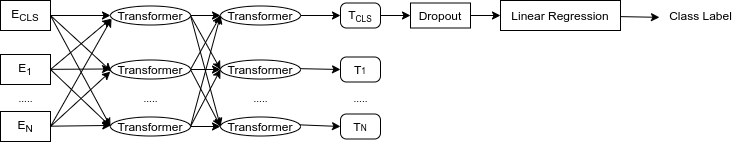
\includegraphics[width= 0.9\textwidth]{gambar/bert_arch.png}
        \caption{The Architecture of BERT in this research}
        \label{fig: bert_arch}
    \end{center}
\end{figure*}

In this research, we decided to use fine-tuning approach, what this mean is that we use a pre-trained BERT model rather than create our own BERT model from scratch, however, we still need to connect the last layer of BERT into a classification layer. In this case, we chose Linear Reggression as the classification layer. For greater detail, figure \ref{fig: bert_arch} is the architecture of BERT that will be used throughout this research.

\subsection{Training and Validation}

\begin{figure}[h!]
    \begin{center}
        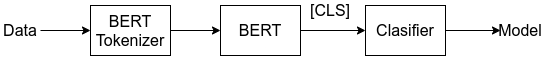
\includegraphics[width= 0.9\linewidth]{gambar/training.png}
        \caption{Training Method}
        \label{fig: metodologi_training}
    \end{center}
\end{figure}

At this stage, the raw text that will be inputted into BERT has already going through its preprocessing phase and is now going into a process called Tokenizer. Tokenizer is a process to change words in a text into token according to its word embedding that is already obtained beforehand when BERT is still in its pretraining phase. Only after all of these process has done, BERT will start its training phase based on the tokenized and preprocessed data.

Not all of the output of the BERT is being used in this particular research, we only need the content of the \texttt{[CLS]} token that is filled with the pooled output of all the other tokens and layers. The content of the \texttt{[CLS]} token is then inputted into Linear Regresson method. This method is choosen as it is easy enough while still retain quite good accuracy. Figure \ref{fig: metodologi_training} is the training method in a nutshell.

There are also some parameters that we can adjust only in this stage, namely batch, learning rate, and epoch. Batch is a parameter to adjust how much data is being processed at once per iteration, mind you that there are usually a few iteration per epoch. By adjusting the batch values, the higher it is, the faster the training process is but at the cost of the memory usage. Thanks to BERT method having quite a large number of layers (718 layers, in general) it can be considered quite heavy, hence we are set the batch value at 10.

Epoch is how much training and validation will take place before the training phase is considered as final. This parameter is one of the most important parameters to adjust as it has a direct effect on the accuracy and the loss of our model. If our loss is too high but the accuracy is too low, it is a clear indication that our model is suffering from underfitting state, meanwhile, if our loss is too low while the accuracy is too high we still need to check if our model is actually good or if it is suffering from overfitting. As our goals in this research is only to process text that is considered to be easier compared to processing image or video, we only set the epoch value to 10.

Learning rate is how much hyperparameter is allowed to change while the model is still in training process, this in turn will change the weight of the layers while in the same process based on the feedback gotten from validation phase. We decided to use the recommended value of 0.00002 \cite{koto2020indolem}

The validation process is used as a way to get the loss validation value that we can use as a comparator between the loss value that we are able to obtain from the training process and the loss validation value that we get from this process. If the loss validation value is getting higher but coupled with a loss training value that shows sign of going lower still, it is a surefire way to know that our model is suffering from overfitting. In another note, if both of our loss value in our model is quite high, then there is a high chance our model is underfitting. Both cases indicate that our model can be further optimized and requiring more training while adjusting the parameter.

\subsection{Testing}

After going through validation and training phase, lastly, we need to test our newly created model. Based on the result of this process, we should be able to conclude whether our model can be considered good enough for our use case, or still can be further adjusted by reconfiguring some of the parameters back at the training phase.

\subsection{Performance Analysis}

The last step right after testing is performance analysis on our tested model. This process is quite important to see how our model will fare in real world scenario after it is being implemented. There are a few metrics that we are using to do this process, all of these metrics is considered to be the industry standard in the world that is machine learning industry. Firstly, there are confustion matrix to categorize the prediction result based on the actual label in the dataset into 4 division. The division being True Positive (TP), False Positive (FP), True Negative (TN), and False Negative (FN). We also using Recall, Precision, and F1-Score as our performance metrics in this research.